\documentclass[nosignatures]{mscThesis}
% replace the previous line with the next to include a signature page
%\documentclass{mscThesis}
% use the option 'nosignatures' to turn off the signatures page
%\documentclass[nosignatures]{mscThesis}
%
% Thesis data
%-For Confidential Reports, uncomment the next line, if desired change the argument. It is printed on the cover, title page and in the footer per page
%\mscConfidential{CONFIDENTIAL}
%
%-Definition of department, programme, faculty
\mscDepartment{Delft Center for Systems and Control (\textsmaller{DCSC})}%
\mscProgram{Systems and Control}
%Change if needed to
%\mscProgram{Mechanical Engineering}
\mscFaculty{Mechanical, Maritime and Materials Engineering (3mE)}%
%
%-name, date, title
\mscName{J. Random Student}%
\mscDate{\today}%
\mscTitle{Thesis Title}%
\mscSubTitle{Optional Subtitle}%
\mscKeyWords{thesis, msc, subject}% only used in PDF properties
%
%-cover picture
\mscCoverPicture{STYLESTUFF/COVER}% to place a picture ( here the example COVER.eps) on the cover page. Comment out if no picture is to be used
%
%
%-Third party options (create text/logo on the copywrite page)
\mscThirdPartyText{The work in this thesis was supported by Aquaduct Swimming Supplies Incorporated. Their cooperation is hereby gratefully acknowledged.}
\mscThirdPartyLogo{STYLESTUFF/EXAMPLELOGO}
% NOTE: on the title page only the TU Delft logo is permitted.
%
%
% The examination committee  - Supervisors and Readers
\mscSupervisorOne{prof.dr.ir.~M.Y.~Supervisor}
\mscSupervisorTwo{Dr.ir.~M.Y.~Second Super}
%\mscSupervisorThree{}
\mscReaderOne{prof.dr.ir.~M.Y.~First Reader}
\mscReaderTwo{dr.ir.~F.S.T.~Reader-two}
\mscReaderThree{ir.~Th.~Reader-three}
%\mscReaderFour{}
%
% Finalize the thesis data
\setThesisInfo
%
% Use \includeonly{} to build only certain parts of your thesis
%\includeonly{introduction, real_chapter, empty_chapter, long_chapter}%
%
%PH Toegevoegd 24-10-2011
%allow (matlab, C++ etc) listing max 1pt flexibility between lines
\lstset{lineskip=0pt plus 1pt minus 0pt} %%
%
\begin{document}
%
%========================== Front matter ======================================
\frontmatter %
%
% Make the cover page and hell of a lot of title pages
\maketitle
%
%
% Abstract (does not appear in the Table of Contents)
\chapter*{Abstract}%

This research considers using \ac{CoM} height variation as an input for balance control on a humanoid robot. Traditional balance strategies for humanoid robots are taking a step, control of the \ac{CoP} location, a result of the `ankle strategy', and changing the angular momentum about the \ac{CoM}, for example by a `hip strategy'. For humanoid robots, a common assumption behind these strategies is that the \ac{CoM} height is predefined. However, \ac{CoM} height changes can be used as an input for balance control, as for example can be observed during the landing of an athlete after a long jump. 

The first contributions of this work are bounds on the initial states for the \ac{VHIP} from which convergence is possible to a stopped state, also known as capture regions. First, only a unilateral contact constraint is considered; negative \ac{CoM} acceleration cannot be smaller than gravitational acceleration. Second, \ac{CoM} height constraints are added to the model, after which a capture region can still be computed in closed-form. Third, vertical force constraints are added, after which capture regions are computed numerically using a bang-bang control law. The last capture region bridges the transition to the applied part of this work.

The second contribution is a control law on vertical acceleration, suitable for application on a humanoid robot using a momentum-based control framework. Push recovery is tested on NASA's Valkyrie humanoid robot while the robot is standing. In simulation, an increase in recoverable push of $9$\% can be observed when comparing to a controller that only uses \ac{CoP}, when pushing the back of the robot. On hardware, an average increase of $7$\% can be observed for this push direction using a load sensor. Additionally, tests are conducted on hardware on Boston Dynamics' Atlas using a medicine ball on a rope, but no improvement in recovery is observed. The control method for standing push recovery is also extended for use while the robot is walking. For Valkyrie in simulation, recovery improved the most compared with a predefined height approach for a push applied in the first part of the single support state for rear and frontal push directions. Additionally, a hardware result on Atlas while walking is briefly presented.
%
% table of contents, (\toc of \toclof of \tocloflot )
\tocloflot
%
%
%
% Preface
\chapter{Preface}

According to \textsc{WikipediA}, a preface (pronounced ``\emph{preffus}'') is an introduction to a book written by the author of the book. In this preface I can discuss the interesting story of how this thesis came into being. 

This is document is a part of my Master of Science graduation thesis. The idea of doing my thesis on this subject came after a discussion with my good friends Tweedledum and Tweedledee\ldots


%
% Acknowledgements
\chapter{Preface \& Acknowledgments}%
Having a background in mechanical engineering, I have always been motivated in closing the gap between theory and application on a physical system during my master's in control systems. The topic of humanoid robotics offers a very interesting, challenging, platform to dedicate my motivation to. The complex multi-body system of a humanoid robot copes with nonlinearity, hybrid dynamics, actuation limitations and plays with your personal intuition. Also, humanoid robots are still physically far behind of what a human can do, which proves that there is large room for improvement. I believe in the future, substitution of a human with a human-like machine can be a live saving. I believe reaching out to \ac{IHMC} was the best decision to learn from and contribute to this field of research.

I would like to thank \ac{IHMC}, for giving me the opportunity to conduct research at the robotics lab. I am particularly grateful for the supervision that was given to me by Dr. Robert Griffin, Dr. Sylvain Bertrand and Dr. Jerry Pratt. I would like to thank everybody else at the robotics lab for their advice and the joy I experienced of working at the lab. 

I would also like to thank Dr. Javier Alonso-Mora from Delft University of Technology, for supervising me throughout the year I was abroad. Also, I would like to thank the examining committee members Prof. Dr. Martijn Wisse, Committee Member 4 and Committee Member 5.

I would like to thank my mother, father and two brothers, for always being supportive.

\vspace*{15mm}

Delft, University of Technology \hfill \mscname \\
\mscdate
%
% Dedication page. 
\cleardoublepage
\thispagestyle{empty}
\vspace*{\stretch{1}}

% Put your own motto here, or dedicate your work to your Mom or whatever...
\begin{quote}
\noindent``Playing soccer is very simple, but the hardest thing there is, is playing soccer in a simple way.''
	
--- \emph{Johan Cruyff}
\end{quote}

\vspace{\stretch{3}}
\clearemptydoublepage
%
%========================== Main matter ======================================
\mainmatter
%
%
% Introduction
\chapter{Introduction} \label{chap::intro}%
There exist many situations in the world which are not safe, where a human is sent to help. Exploring the terrains of nuclear disasters, searching in a house on fire and clearing mine fields are all examples of this. Technology has extended the human's hand through history to a point where nowadays some people are wondering if we have almost hit the limits of fishing Mother Nature's pond of technology.  Safety standards in both professional and personal environments have greatly improved with the help of knowledge and technology. As is noticeable from the videos of Boston Dynamics going viral all over the world, legged robots, and more specifically humanoid robots, become more in a developed stage. However, comparing with the human physical capabilities, humanoid robots are still at most in a child phase.  The usefulness of these devices and the growth opportunities are a clear motivation to improve them.
\section{Motivation}
The walking humanoid robot system is highly complex. It deals with nonlinear multibody dynamics, complex kinematics, hybrid dynamics between switching ground contacts, unilateral friction-limited contact constraints and actuation limitations. Past research has approached nonlinearities with a linearized description of a walking robot \cite{kajita1992dynamic, pratt2006capture, koolen2012capturability} and has tackled joint level complexities by separating high level and joint level control \cite{kuindersma2016optimization, koolen2016design}. The planning problem of a walking gait has often been tackled by separating the footstep plan from the body motion plan \cite{chestnutt2005footstep,deits2014footstep,englsberger2014trajectory}. Although all these methods break the complexity of the system down and give a better approximation of how it will behave dynamically, often still a lot of assumptions are made. Linearization of the model has the advantage of giving a relatively simple measure, that can have a closed form solution in planning problems and that can be used in linear control. In Figure \ref{fig:3dlipfootinertiaz0} the basic model that is often considered is shown. The robot is modeled as a \ac{LIP} with constant height, were the foot and body inertia can be used for control. Recently research has been done in taking the constant height assumption away \cite{hopkins2014humanoid,liu2015trajectory, koolen2016balance, gao2017increase,nguyen2017dynamic, caron2018capturability}, but application of varying height models in control and planning is not yet proven to be successful. 
\section{Objective}
In this literature survey, the focus is to find how \ac{CoM} height variations are used in dynamic planning and control of a bipedal robot, with the goal of improving the dynamical behavior over rough, but also flat, terrain and improving robustness properties against disturbances. \\
Publications are compared based on several aspects. The needed underlying planning and control strategies for the presented methods play an important role, as they are related to the possibilities of application. The differences between \ac{2D} and \ac{3D} based methods can be pointed out and the differences between methods that require a predefined footstep plan and step timing in contrast to methods that define those. Computation times of the methods are compared, as they play an important role in real-time use. Presented results can be evaluated on the contribution to theory and application, where improvements or differences with respect to existing approaches are pointed out. In the case of control, robustness properties of the discussed strategy can be considered. As an example, strategies that fit a predefined footstep plan and that are presented in \ac{3D} are more likely to be applicable than a \ac{2D} strategy that defines the footsteps by the method itself, as most humanoids require a predefined footstep plan and rely on \ac{3D} dynamical models. \\
Even though the research area of focus is exploring the effects of varying height, a global study is done on humanoid robotics research in general, as it is important to understand which strategies are used in aspects that are related to the problem. \\
In Chapter \ref{chap:modeling}, a brief overview is given of basic humanoid walking related models and terminology. In Chapter \ref{chap:planningcontrol}, a general review is conducted on the current planning, control and state estimation strategies in humanoid robotics. Special attention is given to papers that were applied to Boston Dynamics' Atlas or NASA's Valkyrie at IHMC, as research is conducted and hopefully applied at this institute. In Chapter \ref{chap:varyingheight}, a full in-depth study is performed on publications that address \ac{CoM} height variation directly. In Chapter \ref{chap:conclusion}, a conclusion is made on the literature study and a goal for the research project is formulated. Information and ideas from different publications are tied together to attempt to formulate a balanced insight in the possibilities and concerns to tackle the problem.
\begin{figure}[h]
\centering
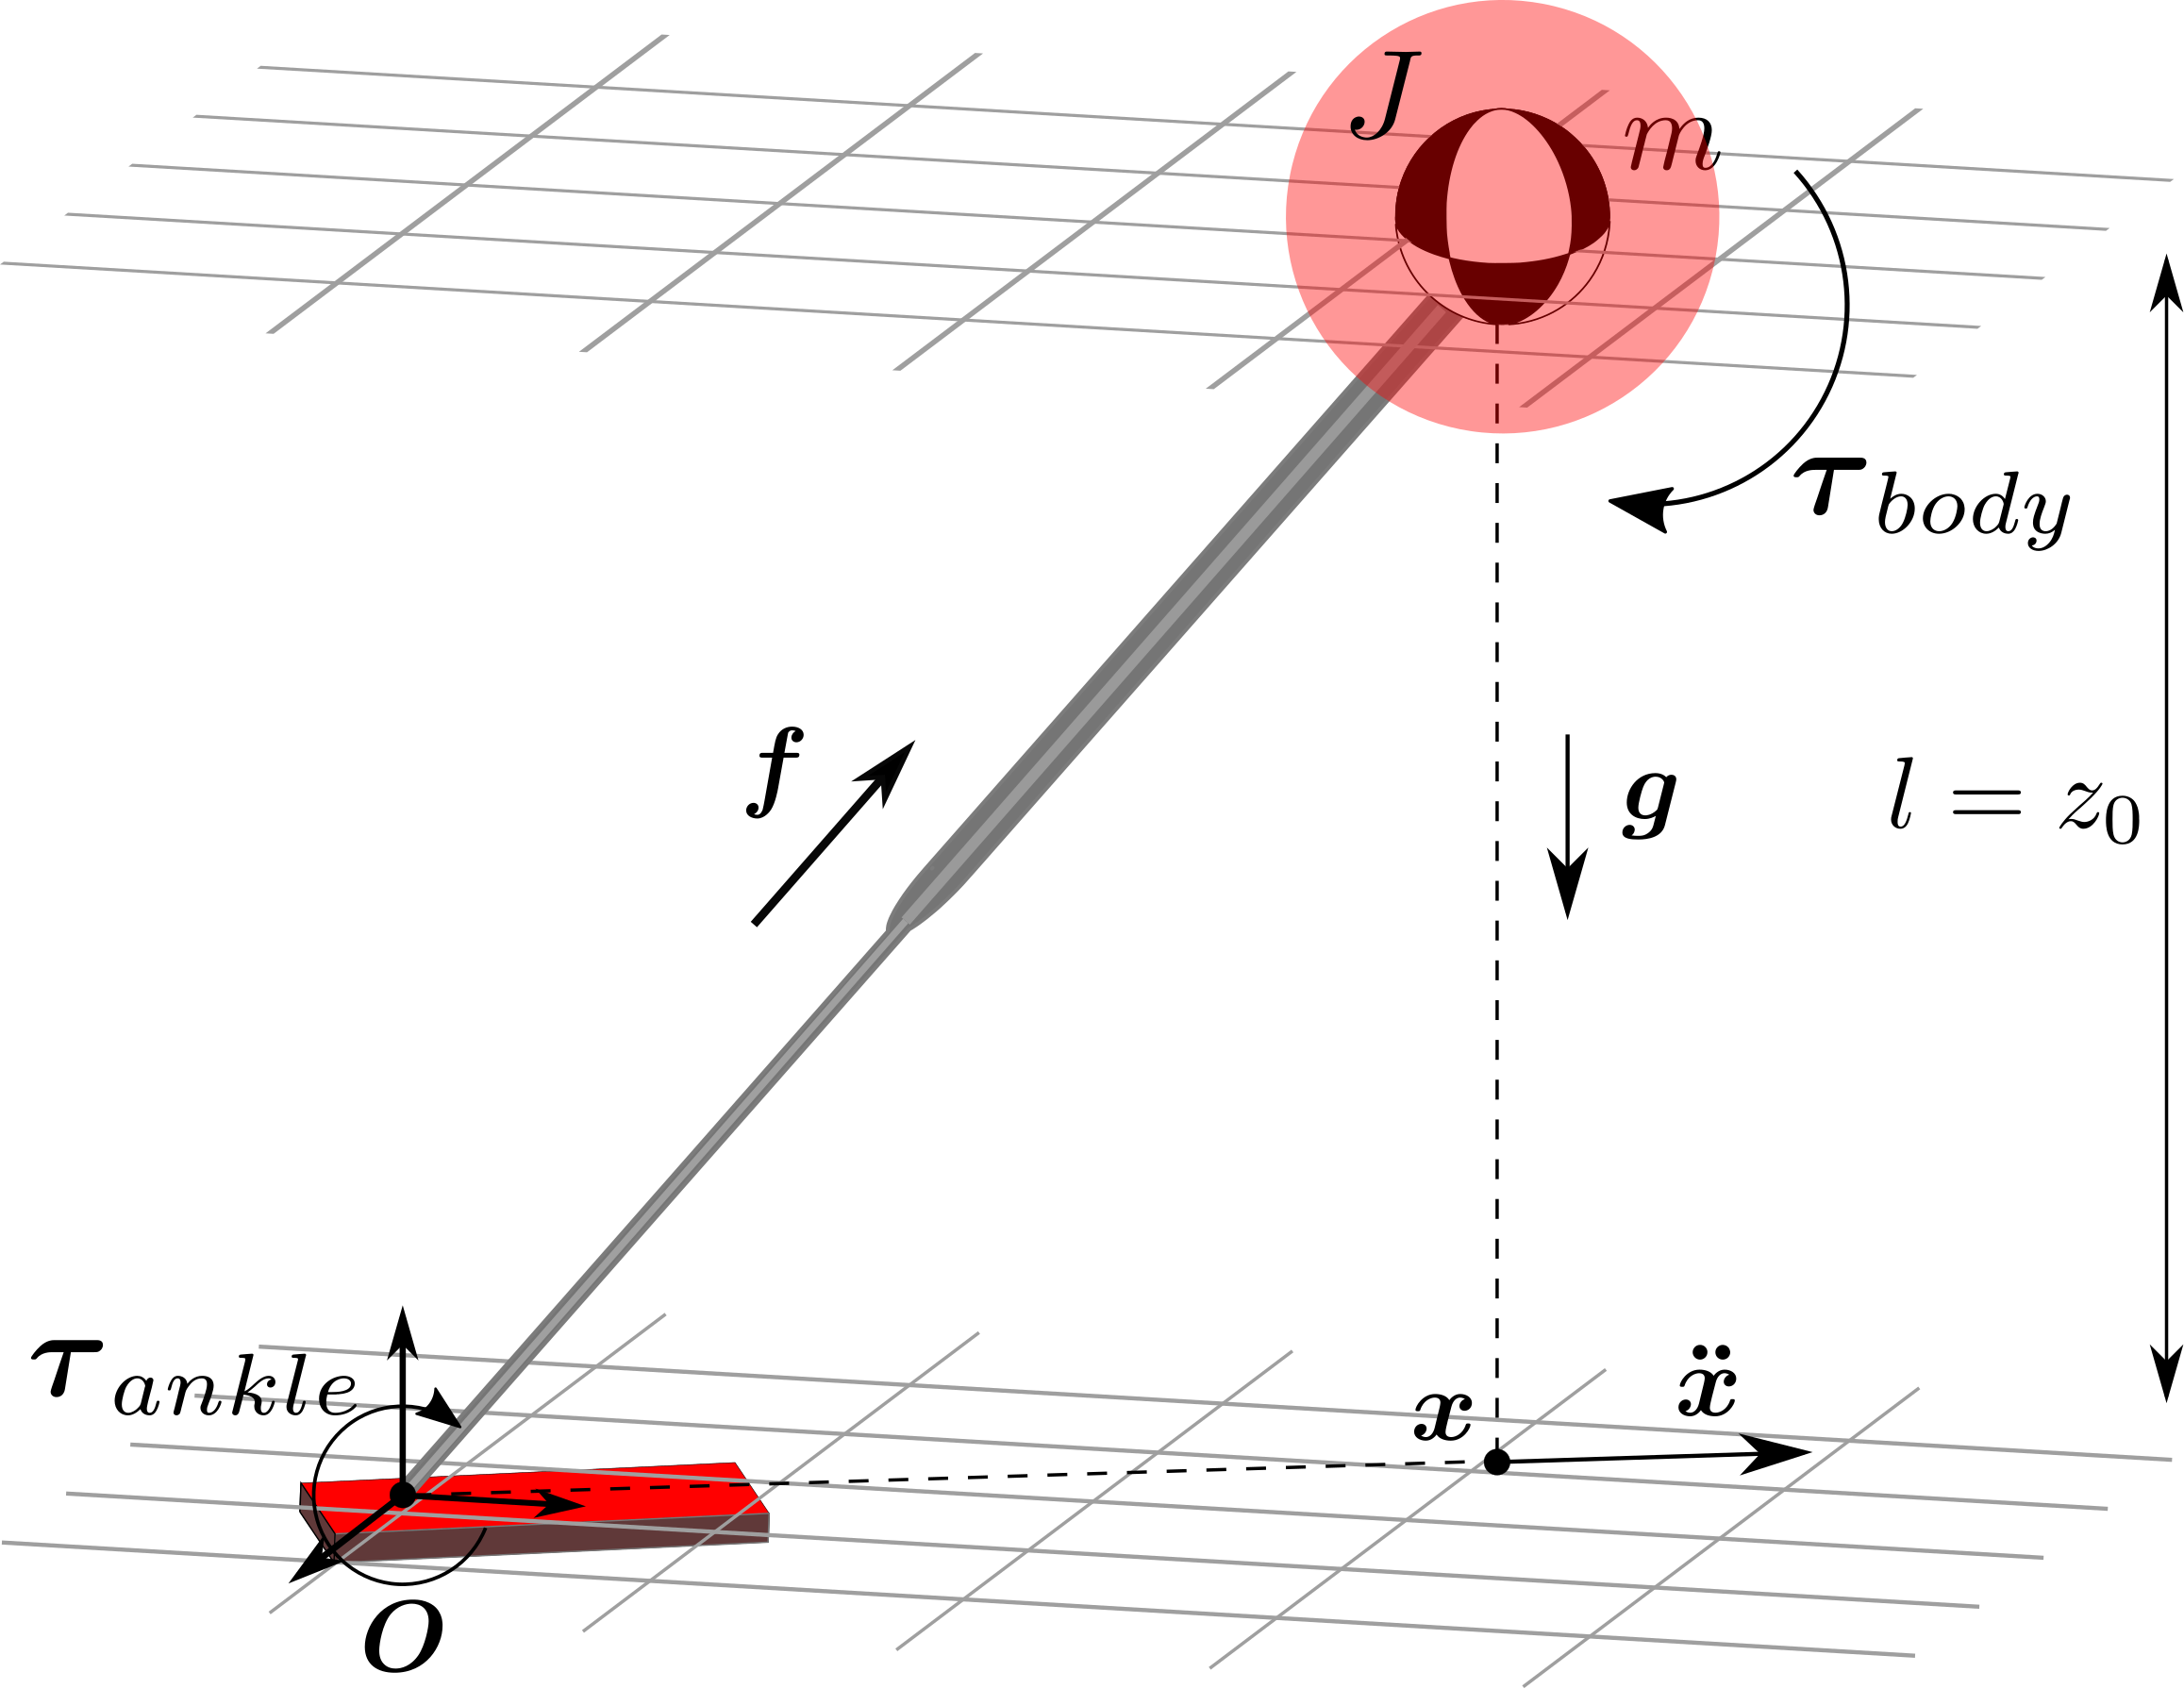
\includegraphics[width=0.5\textwidth]{STYLESTUFF/3DCoMfootinertiaz0.png}
\caption{\ac{3D} motion of \ac{LIP} model with foot at the base and a mass with inertia at the tip. The \ac{CoM} moves at constant height.}
\label{fig:3dlipfootinertiaz0}
\end{figure}





%
% A Real Chapter
\chapter{First Real Chapter}

This is real chapter for \ac{DCSC}, ok? We will use it as a demo for the different headings you can use to structure your text.


\section{First Section}

This is the section. Referring to equations, figures and tables can easily be done by the commands \verb"\eqnref{}", \verb"\figref{}" and \verb"\tabref{}".

\begin{equation}\label{eq:First}
	H(s) = \frac{1}{s+2}
\end{equation}

You see? Refer to equations like this \eqnref{eq:First}.


\subsection{The first subsection}

Subsections are the last type of sectioning that is numbered. 


\subsubsection[Subsection Short Title]{The first sub-subsection with a very very very long title, but in the Table of Contents one can only see the short title}

Quick! Check the Table of Contents! Nice, ain't it?\index{Nice}


\paragraph{A paragraph title}

Subdividing your text in sections and paragraphs automatically makes it nice and structured.
%
% Second chapter
\chapter{Some Basics}

This chapter will cover figures and math. 

\section{Figures}

Figures are constructed using the \texttt{figure} environment:
\begin{verbatim}
\begin{figure}
	\centering
	\includegraphics[options]{imagefile_location}
	\caption{Captions}
	\label{fig:dummy}
\end{figure}
\end{verbatim}

\LaTeX\ automatically decides the best placement of the Figure in your document. This will usually be at the top or bottom of the current page, or at the top of the next page. This system gives good results most of the time, but it can get confused when you have a large number of figures. The command \verb"\clearpage" creates an empty page where any `lost' figures will be printed.

You can refer to a Figure by its label: \verb"\figref{label}". See for instance \figref{fig:dummy}.

\begin{figure}
	\centering
	
\includegraphics[width=0.31415\textwidth]{STYLESTUFF/DCSC}
	\caption{The \acs{DCSC} logo. Pretty nice, eh?}
	\label{fig:dummy}
\end{figure}

\section{Math: \texorpdfstring{$e^{j \pi}=0$}{``Euler's identity''}}

I put some fancy math in the section title. Usually this generates complaints from the \texttt{hyperref} package, because the bookmarks you see on the left can only handle `regular text'. Fortunately, this problem can be solved by using a special command that inserts `regular text' whenever this is necessary during compilation of your thesis: \verb"\texorpdfstring{math}{text}".

For further information about math in \LaTeX, I recommend looking at the Short Math Guide found at \href{http://www.ams.org/tex/amslatex.html}{the website} of the \ac{AMS}. \index{math}

\begin{eqnarray}
% \nonumber to remove numbering (before each equation)
  1 &=& 2\\
  x &=& 5 \\
  y &=& \theta
\end{eqnarray}


\section{More About Acronyms}

After the start of a new chapter all acronyms are reset and are printed as a full acronym the first time it is used again, e.g.\ \ac{DCSC}. After the first use, only the short acronym is printed again: \ac{DCSC}.


\section{More About Nomenclature}

This is a test for nomenclature \lsymb{$A(s)$}{Answer function} \index{test}

%
%
%========================== Appendices =======================================
\appendix
%
%
% An Appendix
\chapter{The Back of the Thesis}

Appendices are found in the back. 


\section{An Appendix Section}

\subsection{An appendix subsection with C++ Listing}

\lstset{language=C++}
\lstinputlisting{test.c}

\subsection{A MATLAB listing}

\lstset{language=matlab}
\lstinputlisting{test.m}

%
% Another appendix chapter
\chapter{Yet Another Appendix}


\section{Test Section (Again?)}

Ok, all is well.


%========================== Back matter ======================================
\backmatter
%
% Bibliography
\bibliographystyle{ieeetr}
\printbib{MyBib}
%
%
% Glossary
\chapter{Glossary} %
%
\printacronyms
\begin{acronym}[\hspace{0.8in}] % 0.8in is also used by the nomenclature
	\acro{3mE}[3\textlarger{m}E]{Mechanical, Maritime and Materials Engineering}%
	\acro{DCSC}{Delft Center for Systems and Control}%
	\acro{ICP}{Instantaneous Capture Point}%
	\acro{CP}{Capture Point}
	\acro{DCM}{Divergent Component of Motion}%
	\acro{ZMP}{Zero Moment Point}%
	\acro{CoP}{Center of Pressure}%
	\acro{CoM}{Center of Mass}%
	\acro{CMP}{Centroidal Momentum Pivot}
	\acro{eCMP}{enhanced Centroidal Momentum Pivot}%
	\acro{VRP}{Virtual Repellent Point}%
	\acro{LIP}{Linear Inverted Pendulum}%
	\acro{2D}{Two-Dimensional Space}%
	\acro{3D}{Three-Dimensional Space}%
	\acro{HZD}{Hybrid Zero Dynamics}%
	\acro{MPC}{Model Predictive Control}%
	\acro{GUI}{Graphical User Interface}%
	\acro{SCS}{Simulation Construction Set}%
	\acro{IMU}{Inertial Measurement Unit}%
	\acro{EKF}{Extended Kalman Filter}%
	\acro{SLIP}{Spring-Loaded Inverted Pendulum}%
\end{acronym}%
%
%
% Nomenclature
\printnomencl%

%
% Index
\cleardoublepage
\printindex

\end{document}
